\chapter{Prior Knowledge Through Augmented Dynamics} \thispagestyle{empty}


\section{Introduction}
Often prior knowledge will come in the form of known, or approximate, relationships between a subset of the system states. An obvious example of this is position-velocity relationships. However, more general problems may be tackled. The task of tracking a reference signal with a given linear combination of states in which the control policy may have access to some preview horizon of the reference can also be tackled by this framework. A further example is non-Markov systems where the system ``state" actually depends on a number of delayed states. All these problems can be tackled using an augmented dynamics model or the use of multiple dynamics models. In order to fit into the probabilistic framework, the use of multiple dynamics must satisfy the propagation of uncertainty criteria outlined in the previous chapter.


\section{Multiple Dynamics Models}
\subsection{Framework}

Consider the case in which the system dynamics function $\bff$ consists of the concatenation of $M$ distinct functions
\begin{equation}
\bff(\bz) = \bff_{1:M}(\bz) := \bmat{\bff_1(\bz) \\ \vdots \\ \bff_M(\bz)}
\label{eqn:multimodel}
\end{equation}
Each sub-function (or sub-dynamics) $\bff_m$ can explicitly depend on any of the previous functional outputs $\bff_{1:m-1}$ as well as the state-action $\bz$. In mathematical terms $\bff_m(\bz) = \bff_m\big(\bz,\bff_{1:m-1}(\bz)\big)$ for $m \in \ZZ_{[2,M]}$. Now define the concatenation of the state-action and the $m-1$ previous functions
\begin{equation}
\bp_m(\bz) = \bmat{\bz \\ \bff_{1:m-1}(\bz) }
\end{equation}
where $\bp_1(\bz) = \bz$.
%
In order to fit into the probabilistic framework of the previous chapter it will be necessary to build up a moment-matched Gaussian approximation $\bff(\bz) \sim \cN(\bm_*, \bS_*)$ given $\bz \sim \cN(\bm,\bS)$. \Ass{gauss} states that $\bm_* = \EE_{\bz,\bff}[\bff(\bz)]$ and $\bS_* = \cov_{\bz,\bff}[\bff(\bz)]$. However, further approximations will have to be made in the case of multiple dynamics models since these moments cannot be calculated for general sub-functions even if the moments of each can be evaluated individually. Therefore \Ass{multigauss} is made.

\begin{ass} \label{ass:multigauss}
In the case of multiple dynamics models the mean $\EE_{\bz,\bff}[\bff(\bz)]$ is composed of blocks $\EE_{\bp_m,\bff_m}\big[\bff_m\big(\bp_m(\bz)\big)\big]$ and the block diagonal of the covariance matrix $\cov_{\bz,\bff}[\bff(\bz)]$ is composed of blocks $\cov_{\bp_m,\bff_m}\big[\bff_m\big(\bp_m(\bz)\big)\big]$ where $\bp_m(\bz) \sim \cN$.
\end{ass}

Therefore, propagation of uncertainty is reduced to the iterative procedure of evaluating the mean $\EE_{\bp_m,\bff_m}\big[\bff_m\big(\bp_m(\bz)\big)\big]$ and covariance $\cov_{\bp_m,\bff_m}\big[\bff_m\big(\bp_m(\bz)\big)\big]$ for each sub-dynamics given the assumed joint Gaussian over the previous values $\bp_m(\bz) \sim \cN$. This is possible provided that these moments can be evaluated for each sub-dynamics.

Now in order to fill out the full covariance matrix $\cov_{\bz,\bff}[\bff(\bz)]$, given \Ass{multigauss}, the cross terms $\cov_{\bp_m,\bff_m}\big[\bff_m\big(\bp_m(\bz)\big), \bp_m(\bz)\big]$ are required. It turns out that if the mean $\EE_{\bp_m,\bff_m}[\bff_m\big(\bp_m(\bz)\big)]$ is differentiable with respect to the input mean $\bm = \EE_{\bp_m}[\bp_m(\bz)]$ then this term can always be evaluated as
%
\begin{align}
\cov_{\bp_m,\bff_m}\big[\bff_m\big(\bp_m(\bz)\big), \bp_m(\bz)\big] &= \bigg(\diff{}{ \bm } \EE_{\bp_m,\bff_m}\big[\bff_m\big(\bp_m(\bz)\big)\big] \bigg) \bS
\label{eqn:multicov}
\end{align}
%
where $\bS = \cov_{\bp_m}[\bp_m(\bz)]$ is the input covariance. This expression holds due to \Theo{inpout}.


\begin{theo}[Output-Input Covariance] \label{theo:inpout}
Consider two random vectors $\ba$ and $\bb$ where $\bb$ is functionally dependent on $\ba \sim \cN(\bm,\bS)$. Then the following statement is true
\begin{equation}
\diff{}{ \bm }\EE_{\ba,\bb}[\bb] =  \cov_{\ba,\bb}[\bb,\ba] \bS^{-1}
\end{equation}
\espa
\end{theo}



\begin{proof}
The proof follows directly from the definition of expectation and covariance
\begin{align*}
\diff{}{\bm}\EE_{\ba,\bb}[\bb]
&= \int \EE_{\bb}[\bb] \bigg( \diff{}{\bm} \cN\big(\ba|\bm,\bS\big) \bigg) \dd\ba  \\
&= \int \EE_{\bb}[\bb] \Big(  (\ba - \bm)\T \bS^{-1} \cN\big(\ba|\bm,\bS\big) \Big) \dd\ba \\
\end{align*}
Now expanding out the brackets yields the expression
\begin{flalign*}
\qquad\qquad\qquad\qquad\quad\;\;
\diff{}{\bm}\EE_{\ba,\bb}[\bb]
&= \bigg( \EE_{\ba,\bb}[\bb \ba\T] - \EE_{\ba,\bb}[\bb] \bm\T \bigg) \bS^{-1}   \\ &
= \cov_{\ba,\bb}[\bb,\ba] \bS^{-1} & \blacksquare
\end{flalign*}
\end{proof}

Note that the assumption of joint Gaussianity is equivalent to assuming linear relationships between sub-dynamics. To see this, observe that \Eq{multicov} is in the form of a Jacobian matrix (or linearised dynamics) multiplied by the input covariance.





\subsection{Subset of Inputs}
Often the case will be that each sub-dynamics is only functionally dependent on a subset, or linear transformation, $\bs_m(\bz)$ of the state-actions and outputs of previous functions $\bp_m(\bz)$. How then is the expectation and covariance with respect to $\bp_m(\bz)$ to be filled in? The answer can be found by considering the general linear transformation $\bs_m(\bz) = \bP_m\bp_m(\bz)$. The matrix $\bP_m$ could either pick off appropriate elements of $\bp_m$ or be viewed as an arbitrary linear combination. Since this mapping is linear, a Gaussian distribution $\bp_m(\bz) \sim \cN(\bm,\bS)$ leads to another Gaussian distribution $\bs_m(\bz) \sim \cN\big(\bm_{\bs},\bS_{\bs}\big)$ with mean $\bm_{\bs} = \bP_m\bm$ and covariance $\bS_{\bs} = \bP_m\bS\bP_m\T$. Therefore the predictive mean and covariance are simply
\begin{align}
\EE_{\bp_m,\bff_m}\big[\bff_m\big(\bp_m(\bz)\big)\big] &= \EE_{\bs_m,\bff_m}\big[\bff_m(\bs_m(\bz)\big)\big] \\
\cov_{\bp_m,\bff_m}\big[\bff_m\big(\bp_m(\bz)\big)\big] &= \cov_{\bs_m,\bff_m}\big[\bff_m\big(\bs_m(\bz)\big)\big]
\end{align}
In order to obtain the cross covariance term $\cov_{\bp_m,\bff_m}\big[\bff_m\big(\bp_m(\bz)\big), \bp_m(\bz)\big] = \cov_{\ba,\bb}[\bb,\ba]$ first define $\bc = \bs_m(\bz)$. Then note that, since $\bb$ is only affected by $\ba$ through $\bc$, the conditional independence relationship $\ba \ci \bb | \bc$ holds. This relationship can be represented by the graphical model shown in \Fig{condind}. Due to the joint Gaussian assumption, \Theo{condind} can be appealed to.






%-------------------------------------------------------------------------------------------------------------------------------------------
\begin{figure}[t]
\centering
%
\tikzstyle{sum} = [circle, draw, minimum height=.8cm]
\tikzstyle{line} = [draw, -stealth']
\begin{tikzpicture}
	\node[sum] (a) at (-2,0) {$\ba$}; 
	\node[sum] (b) at (0,1) {$\bc$};
	\node[sum] (c) at (2,0) {$\bb$};
	\path[line] (a) -- (b); \path[line] (b) -- (c);
\end{tikzpicture}
%
\caption{Graphical model for which the conditional independence relationship $\ba \ci \bb \big| \bc$ holds. See \cite{Bish06} Chapter 8.2 for a more detailed outline.}
\label{fig:condind}
\end{figure}
%-------------------------------------------------------------------------------------------------------------------------------------------





\begin{theo}[Conditional Independence] \label{theo:condind}
Take three random vectors $\ba,\bb$ and $\bc$ which are jointly Gaussian distributed. Given $\ba \ci \bb | \bc$ the following statement is true
\begin{equation}
\cov[\bb,\ba] = \cov[\bb,\bc] \cov[\bc]^{-1} \cov[\bc,\ba]
\end{equation}
\end{theo}

\begin{proof}
Consider the joint distribution $p(\ba,\bb,\bc)$ partitioned as follows
\begin{equation*}
\bmat{\ba \\ \bb \\ \bc} \sim \cN \left(
\bmat{\bm_{\ba} \\ \bm_{\bb} \\ \bm_{\bc}},
\bmat{
\bS_{\ba} & \bS_{\ba\bb} & \bS_{\ba\bc} \\
\bS_{\bb\ba} & \bS_{\bb} & \bS_{\bb\bc} \\
\bS_{\bc\ba} & \bS_{\bc\bb} & \bS_{\bc}
} \right)
\end{equation*}
Conditioning $\ba$ and $\bb$ on $\bc$ using the identity for a Gaussian conditional distribution yields the cross covariance term
\begin{equation}
\cov[\bb,\ba|\bc] = \bS_{\bb\ba} - \bS_{\bb\bc} \bS_{\bc}^{-1} \bS_{\bc\ba}
\end{equation}
This expression is equal to zero since the conditional independence relationship $\ba \ci \bb | \bc$ can be stated equivalently as $\cov[\ba,\bb|\bc] = \bO$. The result follows from a rearrangement of terms.
\qed
\end{proof}

However, computing the inverse of the potentially singular matrix $\cov[\bc]$ is unsatisfactory. Fortunately, explicit calculation of this inversion is unnecessary since $\cov[\bb,\bc] \bS_{\bs}^{-1} = \dd\EE[\bb]/\dd\bm_{\bs}$ due to \Theo{inpout}. Therefore the cross covariances can be expressed as
\begin{align}
\cov_{\bp_m,\bff_m}\big[\bff_m\big(\bp_m(\bz)\big), \bp_m(\bz)\big]
&= \bigg(\diff{}{ \bm_{\bs} } \EE_{\bs_m,\bff_m}[\bff_m\big(\bs_m(\bz)\big)\big] \bigg) \bP_m \bS
\end{align}
where $\bP_m\bS = \cov[\bc,\ba]$. This concludes the definition of the framework for propagation of Gaussian uncertainty given multiple dynamics models of the form given in \Eq{multimodel}. Note that the only condition on each sub-dynamics is that the mean $\EE_{\bs_m,\bff_m}\big[\bff_m\big(\bs_m(\bz)\big)\big]$ and covariance $\cov_{\bs_m,\bff_m}\big[\bff_m\big(\bs_m(\bz)\big)\big]$ are analytically tractable for $\bs_m \sim \cN$, $\bff_m \sim \mathcal{GP}$ and that the mean is differentiable with respect to the mean of the input distribution $\bm_{\bs}$. Now some specific applications are discussed.


\subsection{$N$th Order Markov Systems} \label{sec:nonmarkov}
One use of this framework that is immediately transparent is the case in which the system in question has a Markov order greater than 1 in its relationship to previous states. In other words, with multiple dynamics models, $N\tth$-order Markov systems of the form
\begin{equation}
\bx_k = \bff\big(\bx_{k-1},\bu_{k-1}\dots\bx_{k-N},\bu_{k-N}\big)
\end{equation}
can be considered by defining the augmented state-space system
\begin{equation}
\bx^{\aug}_k = \bmat{ \bff\big(\bx^{\aug}_{k-1},\bu_{k-1}\big) \\[0.1cm] 
\bx_{k-1} \\
\bu_{k-1} \\
\big[\bO_{}, \bI, \bO\big] \bx^{\aug}_{k-1}
}
\end{equation}
with augmented state $\bx^{\aug}_k = [\bx_{k}; \bx_{k-1}; \bu_{k-1} \dots \bu_{k-N};  \bx_{k-N}] \in \RR^{E+ND}$. This is a useful property that will be exploited in the subsequent sections.







\section{Known State Relationships}

\subsection{General Mappings}
The framework of multiple dynamics models outlined in the previous section finds one of its most useful applications in the incorporation of known relationships between states, a form of partial model information. This application is presented in \cite{HRM12}. Specifically, given a system composed of $M$ distinct functions as given in \Eq{multimodel}, then often some of the sub-dynamics may be fixed or known beforehand. In this case, the unknown dynamics can be inferred from data using a parametric or nonparametric method outlined in \Sec{bayesmodelling} while the known parts can be included directly. A very clear and useful example of this for dynamical systems is the case where some states are known to be time derivatives of other states. In other words, position-velocity relationships.



\subsection{Position-Velocity}
\label{sec:posvel}




Consider the common scenario in which the state $\bx$ contains \textit{position} states $\bxp$ and \textit{velocity} states $\bxv$ which are related through
\begin{align}
\bxp_k &= \int_{-\infty}^t \!\!\!\!\bxv(\tau) \dd\tau \quad\text{or}\quad
\bxp_k = \bxp_{k-1} + \int_{t-\Dt}^t \!\!\!\!\bxv(\tau) \dd\tau \label{eqn:posint} \\[0.2cm]
\bxv_k &= \frac{\dd\bxp(\tau)}{\dd \tau} \bigg|_{\tau = t} \label{eqn:veldiff}
\end{align}
where $k \in \ZZ$ and $t = k\Dt$. In order to incorporate this information into the learning framework it is important to first determine whether a predictive model for the position states is to be inferred and the velocity states reconstructed from this prediction (numerical differentiation) or vice versa (numerical integration). Approximate solutions for both cases will be discussed.

First consider the reconstruction of the position states $\bxp_k$ given the previous position $\bxp_{k-1}$ and the set of inferred velocities $\bxv_k$ and $\bxv_{k-1}$ from the probabilistic model. This corresponds to approximating the integral in \Eq{posint} which is depicted graphically in \Fig{posint}. Assuming the velocity follows a constant or linear variation (equivalently the acceleration is zero or constant across the interval) corresponds to the following approximations
\begin{align}
\bxp_k &\approx \bxp_{k-1} + \Dt\bxv_k \label{eqn:int1} \\
\bxp_k &\approx \bxp_{k-1} + \tfrac{1}{2} \Dt \Big( \bxv_k + \bxv_{k-1} \Big) \label{eqn:int2}
\end{align}
respectively. These are roughly equivalent to the Euler and Heun methods for numerical integration. Now consider reconstruction of the velocity states $\bxv_k$ given the inferred velocities $\bxp_k$ and $\bxp_{k-1}$. In this case assuming the position follows a linear or quadratic variation (equivalently the acceleration is zero or constant across the interval) leads to
\begin{align}
\bxv_k &\approx \Dt\inv \Big( \bxp_k - \bxp_{k-1} \Big) \label{eqn:diff1} \\
\bxv_k &\approx 2 \Dt\inv \Big( \bxp_k - \bxp_{k-1} \Big) - \bxv_{k-1} \label{eqn:diff2}
\end{align}
respectively. This process is depicted in \Fig{veldiff}. As expected, these relationships are simply rearrangements of \Eqs{int1}{int2}. All these approximate relationships are linear and can therefore be easily incorporated into the multiple dynamics framework.







%-------------------------------------------------------------------------------------------------------------------------------------------
\begin{figure}[t]
\centering
%
\subfigure[Integral approximations.]{
\tikzstyle{line} = [draw, -stealth']
\begin{tikzpicture}
	\small
	\node at (0,0) {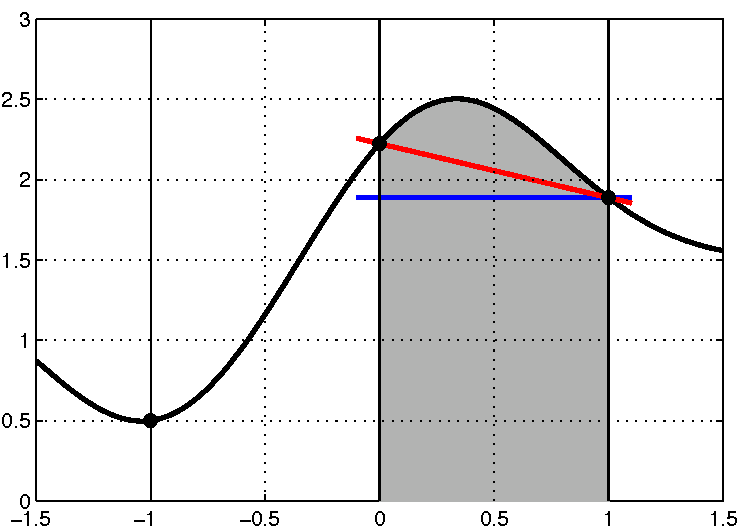
\includegraphics[scale=0.61, clip, trim=0cm 0cm 0cm 0.2cm]{figs/prioraug/vp1.pdf}};
	\path[line] (-3.55,-2.45) -- (3.55,-2.45); \path[line] (-3.45,-2.55) -- (-3.45,2.5);
	\node at (2.3,-2.8) {$t$}; \node at (3.2,-2.75) {time};
	\node at (0,-2.8) {$t-\Dt$};
	\node at (-2.3,-2.8) {$t-2\Dt$};
	\node[rotate=90] at (-3.05,1.65) {velocity $\bxv$};
	\node at (1.2,-1) {$\int_{t-\Dt}^t \bxv \dd\tau$};
\end{tikzpicture}
\label{fig:posint}
}
%
\subfigure[Derivative approximations.]{
\tikzstyle{line} = [draw, -stealth']
\begin{tikzpicture}
	\small
	\node at (0,0) {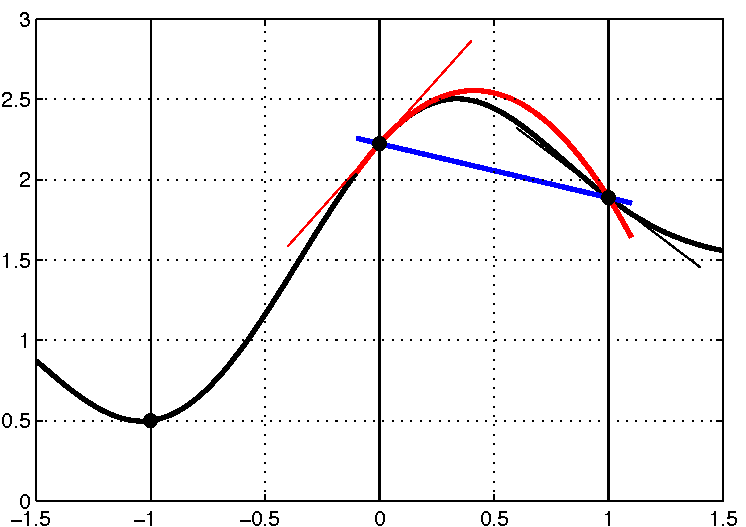
\includegraphics[scale=0.61, clip, trim=0cm 0cm 0cm 0.2cm]{figs/prioraug/vp2.pdf}};
	\path[line] (-3.55,-2.45) -- (3.55,-2.45); \path[line] (-3.45,-2.55) -- (-3.45,2.5);
	\node at (2.3,-2.8) {$t$}; \node at (3.2,-2.75) {time};
	\node at (0,-2.8) {$t-\Dt$};
	\node at (-2.3,-2.8) {$t-2\Dt$};
	\node[rotate=90] at (-3.05,1.65) {position $\bxp$};
	\node at (3.2,-0.4) {$\frac{\dd\bxp}{\dd \tau}(t)$};
\end{tikzpicture}
\label{fig:veldiff}
}
%
\caption{Approximate reconstruction of the current position/velocity states given previous observations of the velocity/position states up to time $t-\Dt$. The blue and red plots in each plot make approximation of zero and constant acceleration $\dot\bxv$ respectively. }
\end{figure}
%-------------------------------------------------------------------------------------------------------------------------------------------


%-------------------------------------------------------------------------------------------------------------------------------------------
\begin{figure}[t]
\centering
%
\subfigure[Integral approximations.]{
\tikzstyle{line} = [draw, -stealth']
\begin{tikzpicture}
	\small
	\node at (0,0) {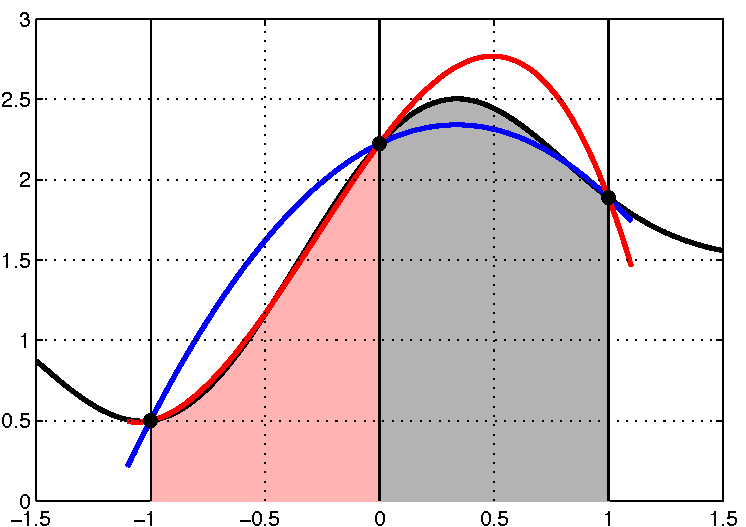
\includegraphics[scale=0.61, clip, trim=0cm 0cm 0cm 0.2cm]{figs/prioraug/vp3.pdf}};
	\path[line] (-3.55,-2.45) -- (3.55,-2.45); \path[line] (-3.45,-2.55) -- (-3.45,2.5);
	\node at (2.3,-2.8) {$t$}; \node at (3.2,-2.78) {time};
	\node at (0,-2.8) {$t-\Dt$};
	\node at (-2.3,-2.8) {$t-2\Dt$};
	\node[rotate=90] at (-3.05,1.65) {velocity $\bxv$};
	\node at (1.2,-1) {$\int_{t-\Dt}^t \bxv \dd\tau$};
\end{tikzpicture}
\label{fig:posint2}
}
%
\subfigure[Derivative approximations.]{
\tikzstyle{line} = [draw, -stealth']
\begin{tikzpicture}
	\small
	\node at (0,0) {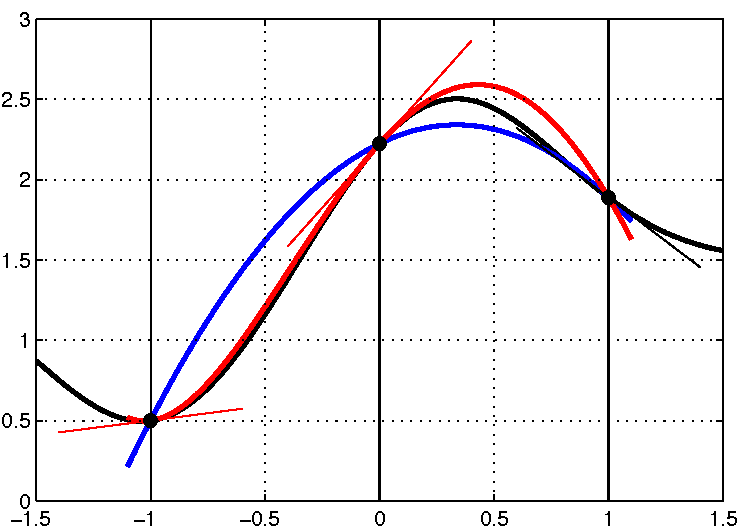
\includegraphics[scale=0.61, clip, trim=0cm 0cm 0cm 0.2cm]{figs/prioraug/vp4.pdf}};
	\path[line] (-3.55,-2.45) -- (3.55,-2.45); \path[line] (-3.45,-2.55) -- (-3.45,2.5);
	\node at (2.3,-2.8) {$t$}; \node at (3.2,-2.78) {time};
	\node at (0,-2.8) {$t-\Dt$};
	\node at (-2.3,-2.8) {$t-2\Dt$};
	\node[rotate=90] at (-3.05,1.65) {position $\bxp$};
	\node at (3.2,-0.4) {$\frac{\dd\bxp}{\dd \tau}(t)$};
\end{tikzpicture}
\label{fig:veldiff2}
}
%
\caption{Approximate reconstruction of the current position/velocity states given previous observations of the velocity/position states up to time $t-2\Dt$. The blue line in plot (a) and (b) use only the three observed points on the graph to make a quadratic approximation of the actual curve. The red line in plot (a) additionally uses the red shaded area $\int \bxv \dd\tau$ over $[t-2\Dt,t-\Dt]$ to form a cubic approximation. This is equivalent to the red line in plot (b) which uses the derivatives $\frac{\dd\bxp}{\dd \tau}(t-\Dt)$ and $\frac{\dd\bxp}{\dd \tau} (t-2\Dt)$ shown by thin red lines to make a quartic approximation.}
\label{fig:posvel2}
\end{figure}
%-------------------------------------------------------------------------------------------------------------------------------------------





As discussed in \Sec{nonmarkov} it is not a problem to form dependencies on delayed states $\bx_{k-i}$ for $i >1$. Therefore, more elaborate approximations can be made by using information from previous timesteps. For example, fitting a quadratic curve to the points $\bxv_k, \bxv_{k-1}, \bxv_{k-2}$ or fitting a cubic curve to these points and given the area defined by $\bxp_{k-1} - \bxp_{k-2}$ yields the following approximations
\begin{align}
\bxp_{k} &\approx \bxp_{k-1} + \tfrac{1}{12}\Dt\Big( 5\bxv_k + 8\bxv_{k-1} - \bxv_{k-2} \Big) \label{eqn:dada} \\
\bxp_{k} &\approx \bxp_{k-2} + \tfrac{1}{3}\Dt\Big( \bxv_k + 4\bxv_{k-1} + \bxv_{k-2} \Big) \label{eqn:mama}
\end{align}
for position reconstruction. These approximations are shown in \Fig{posint2} by the blue and red curves respectively. Note that since there are four constraints that must be satisfied then a cubic function can do this uniquely since it has four degree of freedom. Lower order polynomials could also be considered which would yield a unique analytic solution but would not guarantee satisfaction of the constraints.

Now, in terms of velocity reconstruction, a quadratic fit to the points $\bxp_k, \bxp_{k-1}, \bxp_{k-2}$ and a quartic fit to these points plus the derivatives defined by $\bxv_{k-1}$ and $\bxv_{k-2}$ which give the relationships
\begin{align}
\bxv_{k} &\approx \tfrac{1}{2} \Dt\inv \Big( 3\bxp_{k} - 4\bxp_{k-1} + \bxp_{k-2} \Big) \label{eqn:dada2} \\
\bxv_{k} &\approx 3\Dt\inv \Big( \bxp_k - \bxp_{k-2} \Big) - \Big( 4\bxv_{k-1} + \bxv_{k-2} \Big) \label{eqn:mama2}
\end{align}
Note that the cubic fit to the velocity profile in \Eq{mama} is equivalent to the quartic fit to the position profile in \Eq{mama2}. These approximations are shown in \Fig{veldiff2} by the blue and red curves respectively.

It is important to note that using additional information from previous timesteps and higher order polynomials will not necessarily give better approximations of the integral or derivative. This is clearly shown in \Fig{posvel2} where the higher order polynomial fit (shown in red) produces a poorer approximation of the required integral and derivative in both instances. The quality of a given approximation scheme will therefore be judged by how well it performs in practice.


\subsection{Example: Pendulum} \label{sec:pendulum}

\subsubsection{Setup}
In order to analyse these approximation schemes, the torque-limited pendulum swing up problem was considered. This simple system is shown in \Fig{pendulum} where the pendulum is considered to be a pole of uniform density. The equation of motion for this system is
\begin{equation}
\tfrac{1}{3}ml^2 \ddot{\theta} = u - b\dot\theta - \tfrac{1}{2}mlg\sin\theta,
\end{equation}
with mass $m=1\!$ kg, length $l=1\!$ m, friction $b = 0.1\!$~N$\,$s$^{-1}$, gravitational acceleration $g=9.81\!$~m$\,$s$^{-2}$, states $\bx = [\theta, \dot\theta]^\top$ and constrained input torque $u\in [-3,3]\!$~N$\,$m. This torque is insufficient to swing the pendulum up directly since $u_{max} < \tfrac{1}{2}mlg$.

The cost function used for learning was the angular distance to the upright position $c(\bx) = \half(\cos\theta+1) \in [0,1]$. This cost makes no distinction between swinging the pendulum up to $\theta=\pi$ or $\theta=-\pi$. The prediction horizon was set to $T = 3\!$~s with a discrete timestep $\Delta_t = 0.1\!$ s. Note that this discretisation is relatively short given that the natural period of the pendulum is $T_0 = 2\pi/\omega_0 \approx 1.6\!$~s where $\omega_0 = \sqrt{3g/2l}$.
The control policy was a radial basis function with 50 Gaussian kernels in which the positions, widths and magnitudes of each kernel were free to be optimised. This was then passed through the approximate saturating block defined in \Eq{gsat} in order to satisfy the action constraints. 

The algorithm was given a Gaussian process with a diagonal squared exponential kernel to learn the unknown dynamics. The learned dynamics were then initialised with a training data set of 3$\,$s which was obtained by applying random inputs to the system.

This is an interesting problem since many local minima exist. The optimal solution consists of a single swing back followed by the swing to the upright position, however other solutions may involve multiple swings or swinging the pendulum round and round many times.

%-------------------------------------------------------------------------------------------------------------------------------------------
\begin{figure}[t]
\centering
\input{figs/prioraug/pendulum}
\caption{Torque-limited pendulum with angle from the down position $\theta$, length $l$ and input torque $u$.}
\label{fig:pendulum}
\end{figure}
%-------------------------------------------------------------------------------------------------------------------------------------------



\subsubsection{Standard Method}
The results of applying the standard learning algorithm to the pendulum are shown in \Fig{standi1}. This is clearly an easy task for the algorithm to learn as many runs achieve the task after the first iteration (3$\,$s of data) the majority of runs achieve the swing up task by the second iteration (6$\,$s of data). What makes this an interesting problem is not the learning speed but that there are clearly three solutions that the algorithm gets stuck in. These are shown in \Fig{standj1}. The first, shown in blue, is an ideal solution consisting of a single-swing back before the swing-up. This is close to the theoretical limit, shown by the thin red line and determined through dynamic programming. It is desirable for all runs to end up here. The second mode, shown in black, is a locally optimal solution consisting of two swings before the swing-up. Finally, there is a common failure mode shown in red in which the policy simply applies the maximum control action over the whole horizon and gets stuck here.

The distribution of the predicted expected costs are also given in \Fig{standi1} by the dashed line. These correspond relatively closely to the actual performance with the exception that they almost invariably underestimate how well it will perform. This discrepancy can be assigned to the fact that the variance in the predictions will lead to conservativeness in the predictions. 







%-------------------------------------------------------------------------------------------------------------------------------------------
\begin{figure}[t!]
\centering \footnotesize
\subfigure[Distribution of costs after each iteration]{
\tikzstyle{sum} = [rectangle, draw, rounded corners, minimum height=0.35cm, text width = 0.7cm]
\begin{tikzpicture}
  \node at (0,0) {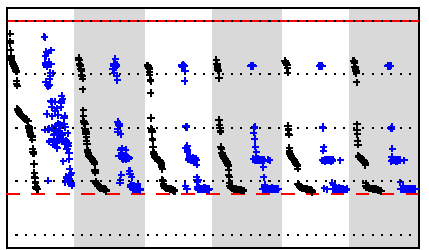
\includegraphics[scale = 0.85]{figs/prioraug/intdiff_heu1.pdf}};
  \node at (0,-2.3) {Algorithm Iteration};
  \node[rotate=90] at (-3.65,0.2) {Cost $J^{\bpi}$};
  \node[sum,red,line width=1.5pt] at (2.67,0.7) {};
  \node[sum,black,line width=1.5pt] at (2.67,-0.8) {};
  \node[sum,blue,line width=1.5pt] at (2.67,-1.28) {};
  \node at (0,-2.5) {};
\end{tikzpicture}
\label{fig:standi1}
}
\hspace{1cm}
\subfigure[Three locally optimal solutions]{
\begin{tikzpicture}
  \node at (0,0) {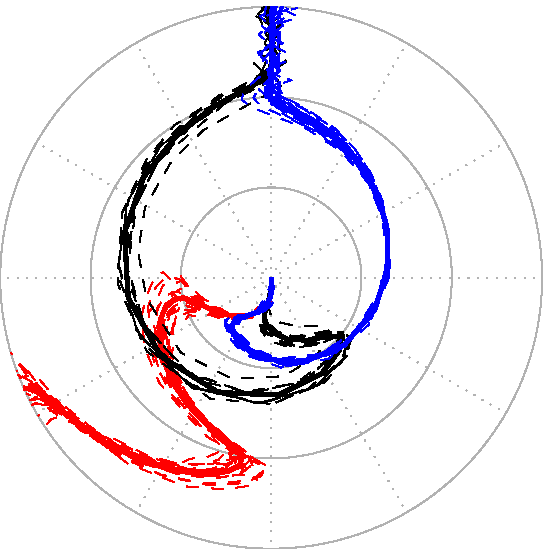
\includegraphics[scale = 0.5]{figs/prioraug/nifty.pdf}};
  \node at (0.65,0.65) {1$\,$s};
  \node at (1.25,1.25) {2$\,$s};
  \node at (1.79,1.79) {3$\,$s};
  \node at (0,-2.55) {down};
  \node at (0,2.55) {upright};
\end{tikzpicture}
\label{fig:standj1}
}
\caption{The graph in (a) depicts the cost trajectories over six iterations of 50 Monte Carlo runs of the standard learning algorithm to the pendulum problem. The black crosses show the actual costs incurred and the blue crosses show the predicted costs. The maximum cost and the global optimum shown by the red line and the red dashed line respectively. The three solutions that the algorithm tended to settle for are shown by the trajectories in (b). The blue is the global optimum solution, consisting of a single swing-back, while the black is a local optimum consisting of two swings. Finally the red is a locally optimal solution of simply applying full actuation torque over the whole horizon.}
\label{fig:stand1}
\end{figure}
%-------------------------------------------------------------------------------------------------------------------------------------------



\subsubsection{The Effect of Uncertainty}
Before moving on to look at the merits of various time-derivative approximation schemes it is first interesting to note the surprising effect that additional predictive uncertainty plays in the context of learning. The graphs in \Fig{noisy} show the results of running the standard algorithm but with an additional injection of predictive uncertainty at each timestep. \Fig{noisy1} shows the effect of applying an artificial additive noise term with distribution $\cN(0,\sigma_{\text{p}}^2)$ to the prediction of $\theta$ at every timestep. Similarly \Fig{noisy2} shows the effect of adding noise with distribution $\cN(0,\sigma_{\text{v}}^2)$ to the prediction of $\dot\theta$.

This process, which would be expected to produce a degradation in performance, in fact produces some surprising results. As shown in the top plot of \Fig{noisy1}, applying additional noise with $\sigma_{\text{p}}^2 = 10^{-1}$ produces some runs that achieve the task with two swings but with the majority of runs entering the failure mode. Uniform improvement of the results with the reduction of this noise term would then be expected to follow. However, as shown by $\sigma_{\text{p}}^2 = 10^{-2}$ this is clearly not the case. Here a significant improvement in performance over the standard method in \Fig{standi1} is observed with all runs achieving the task and most finding the globally optimal solution. In reducing the noise level further the original performance is regained. 

A similar effect can be observed by applying additional noise to the prediction of $\dot\theta$. For $\sigma_{\text{v}}^2 = $ all runs fail the swing up task. However, for $\sigma_{\text{v}}^2 = 10^{-1}$ it can be observed that none of the runs enter the failure mode, but still a significant proportion of the runs getting stuck in the 2-swing solution. Again, reducing the noise level further leads to poorer results.


These results point to an interesting observation about learning systems: Improved performance in learning control can be achieved by treating predictions from a learned model of the system with greater levels of caution than is necessary. The results above show how this principle can be used to help the algorithm not get stuck in locally optimal solutions. However, it is unclear how such a parameter might be tuned therefore it will only be considered in this pendulum example.


%-------------------------------------------------------------------------------------------------------------------------------------------
\begin{figure}[t!]
\centering \footnotesize
\subfigure[Use GPs to learn evolution of both $\theta$ and $\dot\theta$.]{ % Uncertainty in theta
\begin{tikzpicture}
  \node at (5,0) {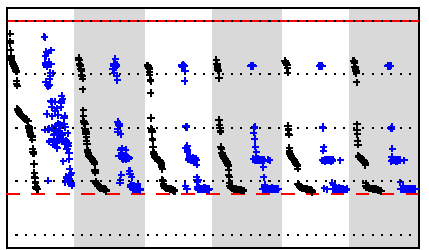
\includegraphics[scale = 0.7]{figs/prioraug/intdiff_heu1.pdf}};
  \node at (0,0) {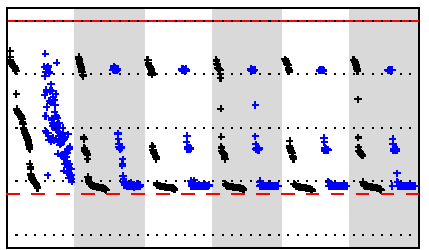
\includegraphics[scale = 0.7]{figs/prioraug/addnoise2.pdf}};
  \node at (-5,0) {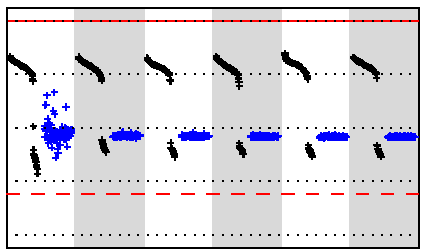
\includegraphics[scale = 0.7]{figs/prioraug/addnoise1.pdf}};
  \node[rotate=90] at (-7.95,0.2) {Cost $J^{\bpi}$};
  \node[fill=white] at (-3.3,1.2) {$\sigma^2 = 0.1$};
  \node[fill=white] at (1.7,1.2) {$\sigma^2 = 0.01$};
  \node[fill=white] at (6.8,1.2) {$\sigma^2 = 0$};
\end{tikzpicture}
\label{fig:noisy1}
} 
\subfigure[Reconstruct $\theta$ using the Euler scheme.]{ % Uncertainty in dtheta
\begin{tikzpicture}
  \node at (5,0) {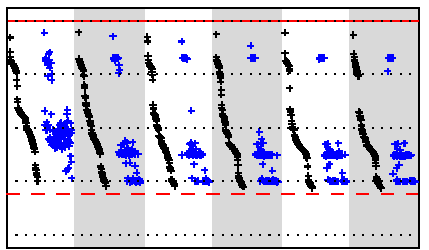
\includegraphics[scale = 0.7]{figs/prioraug/intdiff_eul5.pdf}};
  \node at (0,0) {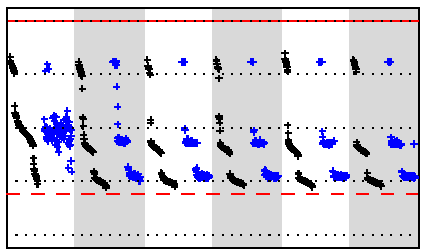
\includegraphics[scale = 0.7]{figs/prioraug/intdiff_eul3.pdf}};
  \node at (-5,0) {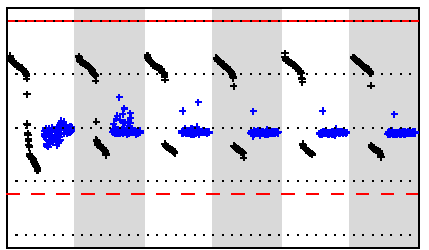
\includegraphics[scale = 0.7]{figs/prioraug/intdiff_eul2.pdf}};
  \node[rotate=90] at (-7.95,0.2) {Cost $J^{\bpi}$};
  \node[fill=white] at (-3.3,1.2) {$\sigma^2 = 0.1$};
  \node[fill=white] at (1.7,1.2) {$\sigma^2 = 0.01$};
  \node[fill=white] at (6.8,1.2) {$\sigma^2 = 0$};
\end{tikzpicture}
\label{fig:eul1}
}
\subfigure[Reconstruct $\theta$ using the Heun scheme.]{ % Uncertainty in dtheta
\begin{tikzpicture}
  \node at (5,0) {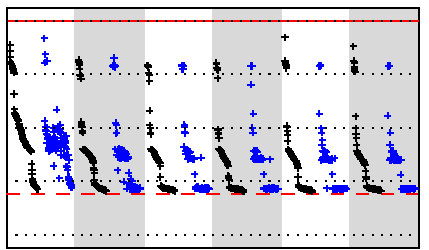
\includegraphics[scale = 0.7]{figs/prioraug/intdiff_heu5.pdf}};
  \node at (0,0) {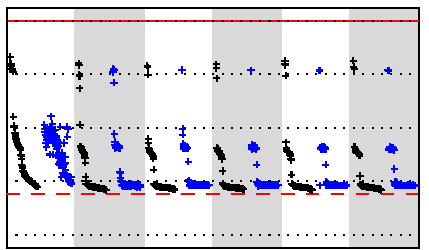
\includegraphics[scale = 0.7]{figs/prioraug/intdiff_heu3.pdf}};
  \node at (-5,0) {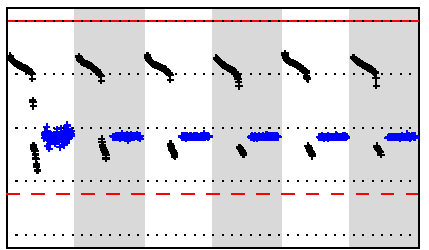
\includegraphics[scale = 0.7]{figs/prioraug/intdiff_heu2.pdf}};
  \node[rotate=90] at (-7.95,0.2) {Cost $J^{\bpi}$};
  \node[fill=white] at (-3.3,1.2) {$\sigma^2 = 0.1$};
  \node[fill=white] at (1.7,1.2) {$\sigma^2 = 0.01$};
  \node[fill=white] at (6.8,1.2) {$\sigma^2 = 0$};
\end{tikzpicture}
\label{fig:heu1}
}
\subfigure[Reconstruct $\theta$ using the 2-step Cubic scheme.]{ % Uncertainty in dtheta
\begin{tikzpicture}
  \node at (5,0) {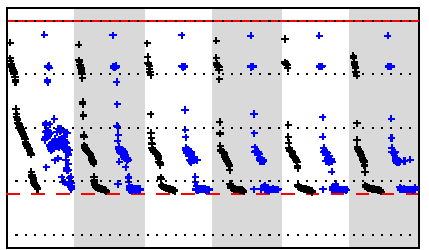
\includegraphics[scale = 0.7]{figs/prioraug/intdiff_fan5.pdf}};
  \node at (0,0) {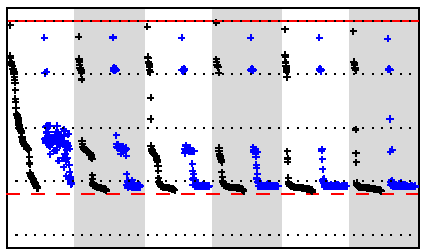
\includegraphics[scale = 0.7]{figs/prioraug/intdiff_fan3.pdf}};
  \node at (-5,0) {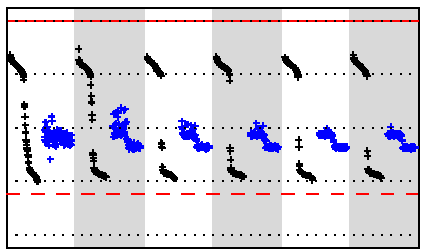
\includegraphics[scale = 0.7]{figs/prioraug/intdiff_fan2.pdf}};
  \node[rotate=90] at (-7.95,0.2) {Cost $J^{\bpi}$};
  \node[fill=white] at (-3.3,1.2) {$\sigma^2 = 0.1$};
  \node[fill=white] at (1.7,1.2) {$\sigma^2 = 0.01$};
  \node[fill=white] at (6.8,1.2) {$\sigma^2 = 0$};
\end{tikzpicture}
\label{fig:fan1}
}
\caption{Plots of the distribution of actual cost (shaded) and the predicted expected cost (dashed) for different levels of additive noise on the prediction of $\theta$ and $\dot\theta$. The x-axis shows the cost $J^{\bpi}$ and the y-axis displays the algorithm iteration. These plots were constructed from 50 Monte Carlo runs with different initial random training data sets.}
\label{fig:integ}
\end{figure}
%-------------------------------------------------------------------------------------------------------------------------------------------


%-------------------------------------------------------------------------------------------------------------------------------------------
\begin{figure}[t!]
\centering \footnotesize
\subfigure[Use GPs to learn evolution of both $\theta$ and $\dot\theta$.]{ % Uncertainty in theta
\begin{tikzpicture}
  \node at (5,0) {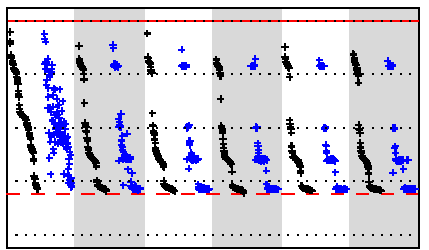
\includegraphics[scale = 0.7]{figs/prioraug/intdiff_fan1.pdf}};
  \node at (0,0) {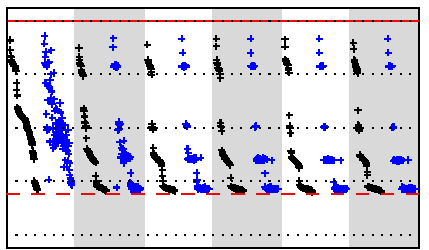
\includegraphics[scale = 0.7]{figs/prioraug/addnoise5.pdf}};
  \node at (-5,0) {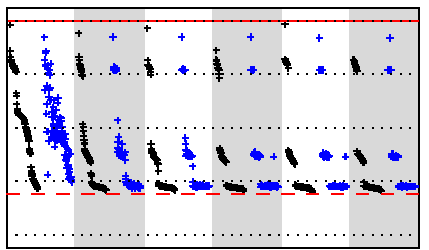
\includegraphics[scale = 0.7]{figs/prioraug/addnoise4.pdf}};
  \node[rotate=90] at (-7.95,0.2) {Cost $J^{\bpi}$};
  \node[fill=white] at (-3.3,1.2) {$\sigma^2 = 0.1$};
  \node[fill=white] at (1.7,1.2) {$\sigma^2 = 0.01$};
  \node[fill=white] at (6.8,1.2) {$\sigma^2 = 0$};
\end{tikzpicture}
\label{fig:noisy2}
} 
\subfigure[Reconstruct $\dot\theta$ using the Euler scheme.]{ % Uncertainty in dtheta
\begin{tikzpicture}
  \node at (5,0) {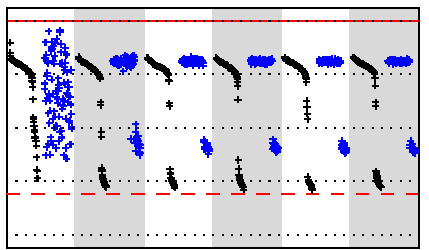
\includegraphics[scale = 0.7]{figs/prioraug/intdiff_eul9.pdf}};
  \node at (0,0) {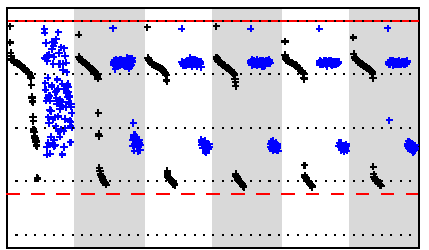
\includegraphics[scale = 0.7]{figs/prioraug/intdiff_eul7.pdf}};
  \node at (-5,0) {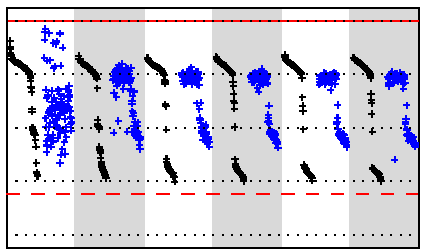
\includegraphics[scale = 0.7]{figs/prioraug/intdiff_eul6.pdf}};
  \node[rotate=90] at (-7.95,0.2) {Cost $J^{\bpi}$};
  \node[fill=white] at (-3.3,1.2) {$\sigma^2 = 0.1$};
  \node[fill=white] at (1.7,1.2) {$\sigma^2 = 0.01$};
  \node[fill=white] at (6.8,1.2) {$\sigma^2 = 0$};
\end{tikzpicture}
\label{fig:eul2}
}
\subfigure[Reconstruct $\dot\theta$ using the Heun scheme.]{ % Uncertainty in dtheta
\begin{tikzpicture}
  \node at (5,0) {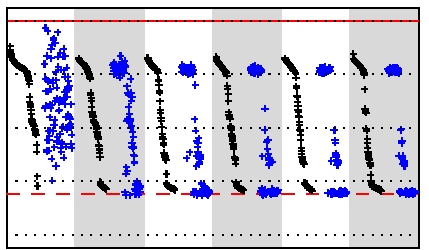
\includegraphics[scale = 0.7]{figs/prioraug/intdiff_heu9.pdf}};
  \node at (0,0) {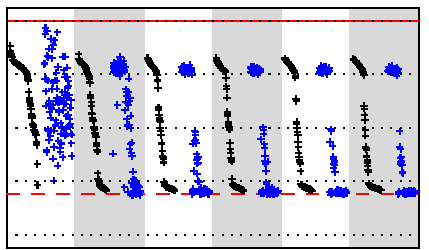
\includegraphics[scale = 0.7]{figs/prioraug/intdiff_heu7.pdf}};
  \node at (-5,0) {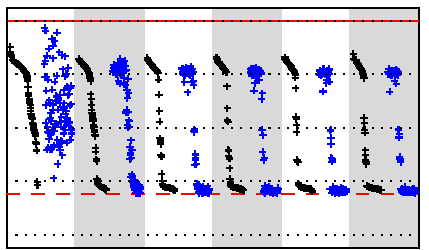
\includegraphics[scale = 0.7]{figs/prioraug/intdiff_heu6.pdf}};
  \node[rotate=90] at (-7.95,0.2) {Cost $J^{\bpi}$};
  \node[fill=white] at (-3.3,1.2) {$\sigma^2 = 0.1$};
  \node[fill=white] at (1.7,1.2) {$\sigma^2 = 0.01$};
  \node[fill=white] at (6.8,1.2) {$\sigma^2 = 0$};
\end{tikzpicture}
\label{fig:heu2}
}
\caption{Plots of the distribution of actual cost (shaded) and the predicted expected cost (dashed) for different levels of additive noise on the prediction of $\theta$ and $\dot\theta$. The x-axis shows the cost $J^{\bpi}$ and the y-axis displays the algorithm iteration. These plots were constructed from 50 Monte Carlo runs with different initial random training data sets.}
\label{fig:differ}
\end{figure}
%-------------------------------------------------------------------------------------------------------------------------------------------





\subsubsection{Position-Velocity Information}
The explicit inclusion of approximate position-velocity information in the pendulum swing-up challenge shall now be considered. The results for a constant acceleration (Heun) approximation are shown in \Fig{intdiff1} for various values of additional additive uncertainty on $\theta$ and $\dot\theta$. Compare the results of \Fig{noisy1} with \Fig{integ1}. The only difference between these is that instead of using a GP to learn a predictive model for $\theta$ the approximate relationship is included directly in the form of \Eq{int2}. It is clear by comparing these plots that the inclusion of this prior knowledge leads to a slight improvement in performance in the sense that a greater number of the runs end up at the global optimum solution for the noise levels $\sigma_{\text{p}}^2 = 10^{-2}$ and $\sigma_{\text{p}}^2 = 10^{-3}$.


The same conclusion can be drawn from including an approximate relationship for reconstructing the velocity term $\dot\theta$. This can be seen by comparing \Fig{noisy2} with \Fig{differ1}. For artificial noise levels of $\sigma_{\text{v}}^2 = 10^{-1}$ and $10^{-2}$ it can be seen that most runs which use this prior information find the global optimum solution. Without this information, there are still a significant number of runs that end up in the locally optimal solution consisting of two swings before the swing up.


What has been observed through these simulations is that inclusion of prior information can help with the problem of falling into locally optimal solutions and give a better chance of finding the global optimum.



Finally, a brief comparison of the various reconstruction methods outlined in \Sec{posvel} will be conducted. The various schemes under consideration will be referred to as the \textit{Euler}, \textit{Heun}, \textit{Quadratic} and \textit{Full 2-step} approximations which will denote \Eq{int1}, \Eq{int2}, \Eq{dada} and \Eq{mama} respectively for position reconstruction and \Eq{diff1}, \Eq{diff2}, \Eq{dada2} and \Eq{mama2} for velocity reconstruction. The results of using these schemes are given in \Fig{intdiff2} where artificial noise levels of $\sigma_{\text{p}}^2 = 10^{-2}$ and $\sigma_{\text{v}}^2 = 10^{-1}$ are used for position and velocity reconstruction respectively since these values yield the best performance for each method.

In each case the Heun method (or constant acceleration approximation) produces the best performance. The Euler method is still a good enough approximation to achieve the task but it does not find as good solutions as the Heun method, or even as the standard method. Looking at the Quadratic approximation, it may be surprising that it does not perform as well, if not better, than the simpler Heun method. For position reconstruction it neither learns the task as fast, and a relatively significant number of the runs end up in the failure mode. Further, the predicted performance is significantly different to the actual performance, indicating that this is actually a poor approximation. For velocity reconstruction it cannot learn the task at all and makes very poor predictions of performance. The results of the Full 2-step approximation has not even been displayed since it cannot learn in either instance.

This is clear evidence that the more elaborate approximations built upon previous approximations do not necessarily give improved performance and in fact can significantly degrade it.









\subsection{Example: Unicycle} \label{sec:unicycle}

\subsubsection{Setup}
The scheme was then tested on a highly nontrivial control problem, the balancing of a robotic unicycle as shown in \Fig{unicycle}. The equations of motion for this system can be found in the thesis of \cite{For09}. The state consists of $\bx = [x_\text{c}, y_\text{c}, \theta, \phi, \psi, \dot\theta, \dot\phi, \dot\psi, \dot\psi_\text{w}, \dot\psi_\text{t}]^\top \in \RR^{10}$ where $(x_\text{c},y_\text{c})$ is the position of the desired unicycle location in a coordinate system centred on the unicycle itself, $\theta$ is the roll angle, $\phi$ is the pitch angle, $\psi$ is the yaw angle, $\psi_\text{w}$ is the angular position of the wheel and $\psi_\text{t}$ is the angular position of the turntable. The action vector is $\bu = [u_\text{t}, u_\text{w}]^\top \in \RR^2$, where $u_\text{t}$ is the torque applied to the turntable and $u_\text{w}$ is the torque applied to the wheel.  and the discrete timestep was set to $\Delta_t = 0.15\!$ s. This is a large timestep given the dynamics of the unicycle and therefore makes the task of control even harder. The prediction horizon was set to $H = \big\lceil 10/\Delta_t \big\rceil$ steps to give a simulation time close to $10\!$ s.

The state measurement was corrupted with white noise of variance $0.002^2\bI$.




%-------------------------------------------------------------------------------------------------------------------------------------------
\begin{figure}[t]
\centering

\begin{tikzpicture}[]

\begin{scope}[canvas is xz plane at y=-1.5]
  \draw[draw=black,fill=black!10,rounded corners] (2.3,2) rectangle (-2.5,-2);
\end{scope}

% origin is (-2.5,-1.5,2)
\draw[thick,blue,-latex'] (-2.7,-1.5,2) -- (-0.5,-1.5,2);
\draw[thick,blue,-latex'] (-2.5,-1.7,2) -- (-2.5,0.5,2);
\draw[thick,blue,-latex'] (-2.5,-1.5,2.3) -- (-2.5,-1.5,-0.8);

\begin{scope}[canvas is xz plane at y=-0.1]
  \draw[rotate=0,-latex',black, thick] (-2.2,2) arc (0:-320:0.3cm);
\end{scope}
\begin{scope}[canvas is xy plane at z=0.1]
  \draw[rotate=0,-latex',black, thick] (-2.25,-1.5) arc (0:-300:0.25cm);
\end{scope}
\begin{scope}[canvas is yz plane at x=-1.1]
  \draw[rotate=0,-latex',black, thick] (-1.2,2) arc (0:300:0.3cm);
\end{scope}

\begin{scope}[canvas is yx plane at z=-0.05]
  \draw[draw=black,fill=black!30,thick,opacity=0.8] (0,0) circle (1.5cm);
\end{scope}
\begin{scope}[canvas is yx plane at z=0.05]
  \draw[draw=black,fill=black!30,thick,opacity=0.8] (0,0) circle (1.5cm);
  \draw[draw=black,fill=black,thick] (0,0) circle (0.1cm);
  \draw[rotate=45,-latex',red, thick] (1.7,0) arc (0:50:1.7cm);
  \draw[rotate=45,-latex', thick] (0.3,0) arc (0:300:0.3cm);
\end{scope}

\draw[line width = 0.05cm] (0,3,0) -- (0,0,0);
\draw[line width = 0.1cm] (0,3,0) -- (0,1.48,0);

\begin{scope}[canvas is xz plane at y=2.94]
  \draw[draw=black,fill=black!30,thick,opacity=0.8] (0,0) circle (1.5cm);
\end{scope}
\begin{scope}[canvas is xz plane at y=3]
  \draw[draw=black,fill=black!30,thick,opacity=0.8] (0,0) circle (1.5cm);
  \draw[draw=black,fill=black,thick] (0,0) circle (0.1cm);
   \draw[rotate=-5,-latex',red, thick] (1.7,0) arc (0:-50:1.7cm);
   \draw[rotate=0,-latex', thick] (0.4,0) arc (0:-300:0.4cm);
\end{scope}


\node at (-0.4,-1.5,2.8) {{\color{blue}$x$}}; \node at (-0.9,-1.2,1.7) {$\theta$};
\node at (-2.1,-1.5,-0.2) {{\color{blue}$y$}}; \node at (-2.5,-1.0,-0.2) {$\phi$};
\node at (-2.2,0.4,2) {{\color{blue}$z$}}; \node at (-2.9,0.2,2) {$\psi$};

\node at (-0.3,-0.6,0) {$\phi_\text{w}$}; \node at (-0.7,3,0.3) {$\psi_\text{t}$};
\node at (1.9,0.7,0) {\color{red}$u_\text{w}$}; \node at (2.3,3.4,0.5) {\color{red}$u_\text{t}$};


\end{tikzpicture}
\caption{Robotic unicycle with roll angle $\theta$, pitch angle $\phi$, yaw angle $\psi$, turntable angle $\psi_{\text{t}}$ and wheel angle $\psi_{\text{w}}$. The controlled inputs are the torque applied to the turntable $u_{\text{t}}$ and the torque applied to the wheel $u_{\text{w}}$.}
\label{fig:unicycle}
\end{figure}
%-------------------------------------------------------------------------------------------------------------------------------------------


\subsubsection{Results}



%-------------------------------------------------------------------------------------------------------------------------------------------
\begin{figure}[t!]
\centering \footnotesize
\subfigure[Use GPs to learn evolution of both $\theta$ and $\dot\theta$.]{ % Uncertainty in theta
\begin{tikzpicture}
  \node at (0,0) {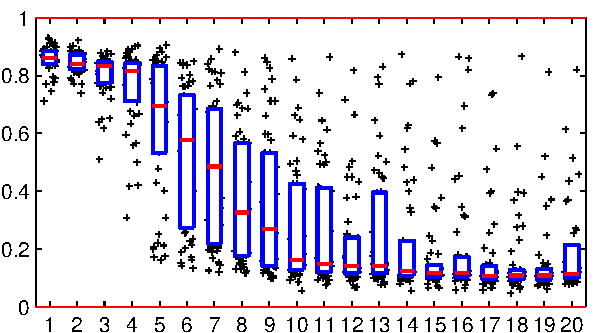
\includegraphics[scale = 0.74]{figs/prioraug/uniplot1.pdf}};
\end{tikzpicture}
\label{fig:unicyc1}
} \hfill
\subfigure[Use GPs to learn evolution of both $\theta$ and $\dot\theta$.]{ % Uncertainty in theta
\begin{tikzpicture}
  \node at (0,0) {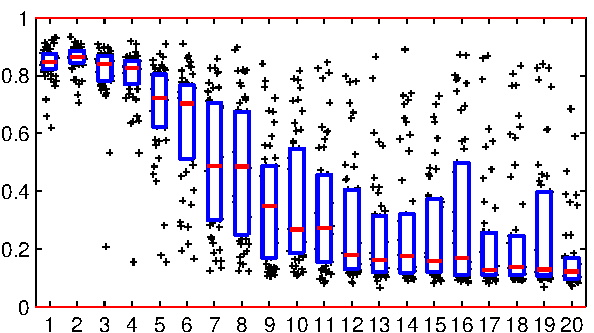
\includegraphics[scale = 0.74]{figs/prioraug/uniplot2.pdf}};
\end{tikzpicture}
\label{fig:unicyc2}
}
\subfigure[Use GPs to learn evolution of both $\theta$ and $\dot\theta$.]{ % Uncertainty in theta
\begin{tikzpicture}
  \node at (0,0) {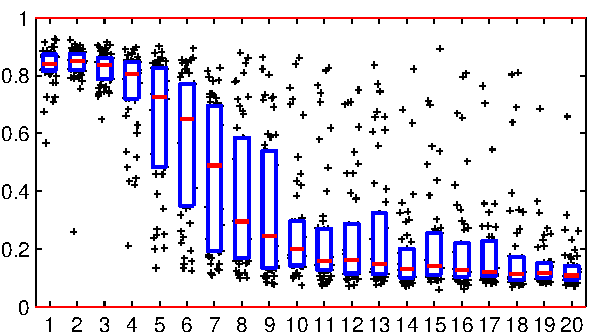
\includegraphics[scale = 0.74]{figs/prioraug/uniplot3.pdf}};
\end{tikzpicture}
\label{fig:unicyc1}
} \hfill
\subfigure[Use GPs to learn evolution of both $\theta$ and $\dot\theta$.]{ % Uncertainty in theta
\begin{tikzpicture}
  \node at (0,0) {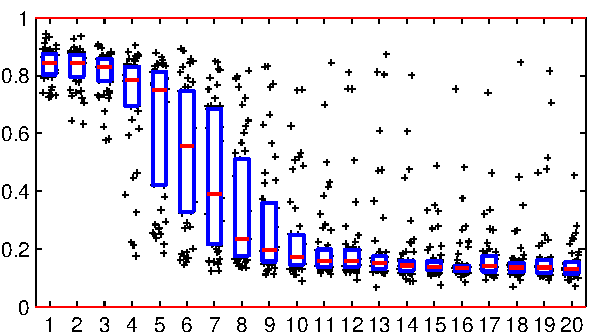
\includegraphics[scale = 0.74]{figs/prioraug/uniplot5.pdf}};
\end{tikzpicture}
\label{fig:unicyc2}
}
\caption{Plots of the distribution of actual cost (shaded) and the predicted expected cost (dashed) for different levels of additive noise on the prediction of $\theta$ and $\dot\theta$. The x-axis shows the cost $J^{\bpi}$ and the y-axis displays the algorithm iteration. These plots were constructed from 50 Monte Carlo runs with different initial random training data sets.}
\label{fig:uniplots}
\end{figure}
%-------------------------------------------------------------------------------------------------------------------------------------------





\section{Reference Tracking}

\subsection{Problem Formulation}
An extension of the regulation problem given by \Eq{Jcost} is now considered. In particular, the problem of forcing a linear combination of the system states $\bC\bx^{\bx}$ to track some reference $\br := \bC^{\br}\bx^{\br}$ where $\bx^{\br} \in \RR^{E_r}$ is the underlying reference state. This will be achieved using a parameterised control policy $\bpi: \RR^{E} \times \RR^{E_r} \rightarrow \RR^F$ which has access to the full reference state.   Mathematically, this problem can be written as
\begin{align}
& \text{minimise} & J^{\bpi} = \EE_{\btau}\Bigg[ & \sum_{k=0}^{H-1} c\big(\bC\bx^{\bx}_k - \bC^{\br}\bx^{\br}_k,\bu_k\big) + c_H\big(\bC\bx^{\bx}_H - \bC^{\br}\bx^{\br}_H\big) \, \bigg| \, p(\bx^{\bx}_0, \bx^{\br}_0) \Bigg]
\label{eqn:reftrack1} \\
&\text{subject to} & \bx^{\bx}_k &= \bff_{\bx}\big(\bx^{\bx}_{k-1},\bu_{k-1}\big) 
\quad \text{where} \quad \bff_{\bx} \sim p\big(\bff_{\bx}|\cD,\hyp\big) & \label{eqn:reftrack2}\\
\nonumber && \bx^{\br}_k &= \bff_{\br}\big(\bx^{\br}_{k-1}\big) \\
\nonumber && \bu_k &= \bpi\big(\bx^{\bx}_k, \bx^{\br}_k \big)
\end{align}
where $\btau := [\bx^{\bx}_0; \bx^{\br}_0; \bu_0 \dots \bx^{\bx}_H]$ is a sampled state-action and reference trajectory. In the spirit of \cite{BGW90}, this problem can be recast as a regulation problem in terms of an augmented state space and dynamics model. First define augmented state as $\bx := [\bx^{\bx}; \bx^{\br}]$. Next define the augmented dynamical system
\begin{equation*}
\bx_{k} =
\bff(\bx_{k-1}, \bu_{k-1}) = \bmat{
\bff_{\bx}\big(\bx^{\bx}_{k-1},\bu_{k-1}\big) \\
\bff_{\br}\big(\bx^{\br}_{k-1}\big)
}
\end{equation*}
and the stage-cost $c^{\br}\big(\bx,\bu\big) := c\big([\bC, -\bC^{\br}]\bx,\bu\big)$. The recast problem can now be stated as a regulation problem in terms of the augmented state space
\begin{align}
& \text{minimise} & J^{\bpi} = \EE_{\btau}\Bigg[ & \sum_{t=0}^{H-1} c^{\br}\big(\bx_k ,\bu_k \big) + c^{\br}_T\big(\bx\big) \, \bigg| \, p(\bx_0) \Bigg]
 \\
&\text{subject to} & \bx_k &= \bff\big(\bx_{k-1},\bu_{k-1}\big) 
\quad \text{where} \quad \bff \sim p\big(\bff|\cD,\hyp\big) & \\
\nonumber && \bu_k &= \bpi\big( \bx_k \big)
\end{align}
which is in exactly the same form as the original regulation problem posed in \Eqs{learn1}{learn2}. Note that if the moments of the stage-cost $c$ are tractable given a Gaussian input $\bx,\bu \sim \cN$ then so will the moments of $c^{\br}$ since the input has only undergone a linear transformation and therefore remains Gaussian.


\subsection{Preview Horizon}
An important point to make is that the problem given in \Eqs{reftrack1}{reftrack2} can handle the situation in which the control policy is allowed to anticipate the impending change in reference by having access to some \textit{preview horizon} of the reference signal. In other words $\bu_k$ is allowed to be functionally dependent on $\br_{k+i}$ for $i \in \ZZ_{[0,H_r]}$ for preview horizon $H_r$ steps. This situation can be encoded by defining the reference state to consist of future values of $\br$ over the preview horizon window $\bx^{\br}_k = [\br_k; \br_{k+1} \dots \br_{k+H_r}]$. Then defining the reference dynamics to consist of
\begin{equation}
\bx^{\br}_k = \bff_{\br}\big( \bx^{\br}_{k-1} \big) = \bmat{
\big[\bO, \bI] \bx^{\br}_{k-1} \\
\bff_{r}(\br_{k+H_r-1})
}
\end{equation}
the problem is back into the form outlined in the previous section. 




\subsection{Reference Dynamics}
\subsubsection{Linear}

%-------------------------------------------------------------------------------------------------------------------------------------------
\begin{figure}[t]
\centering
\tikzstyle{line} = [draw, -stealth']
%
\subfigure[Steps]{
\begin{tikzpicture}
	\footnotesize
	\node at (0,0) {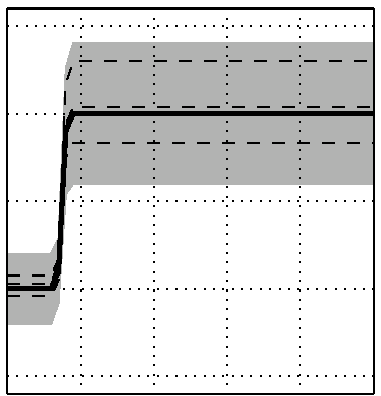
\includegraphics[scale=0.66, clip, trim = .1cm 0cm .1cm 0cm]{figs/prioraug/ref_step.pdf}};
	\node at (0.2,-2.6) {time $(k)$}; \node at (-1.6,2) {$r_k$};
\end{tikzpicture}
\label{fig:linref1}
}
%
\subfigure[Periodic Waves]{
\begin{tikzpicture}
	\footnotesize
	\node at (0,0) {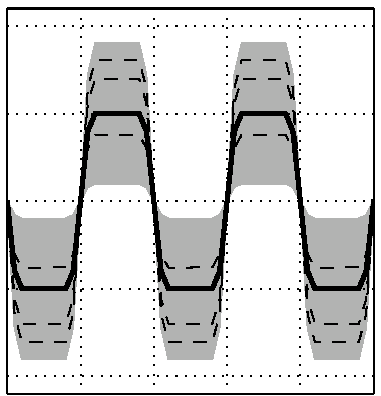
\includegraphics[scale=0.66, clip, trim = .1cm 0cm .1cm 0cm]{figs/prioraug/ref_square.pdf}};
	\node at (0.2,-2.6) {time $(k)$}; \node at (-1.6,2) {$r_k$};
\end{tikzpicture}
\label{fig:linref2}
}
%
\subfigure[Filtered Noise]{
\begin{tikzpicture}
	\footnotesize
	\node at (0,0) {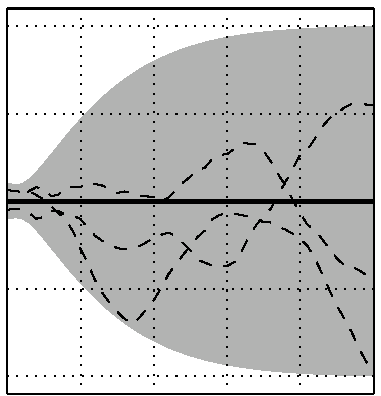
\includegraphics[scale=0.66, clip, trim = .1cm 0cm .1cm 0cm]{figs/prioraug/ref_noise.pdf}};
	\node at (0.2,-2.6) {time $(k)$}; \node at (-1.6,2) {$r_k$};
\end{tikzpicture}
\label{fig:linref3}
}
%
\caption{Examples of reference signals generated from the linear system $\bx^{\br}_k = \bA^{\br}\bx^{\br}_{k-1} + \bb^{\br}e_{k-1}$ where $r_k = [1,\bO]\bx^{\br}$. Plots (a)-(c) were generated using $\bA^{\br}_1, \bb^{\br}_1$, $\bA^{\br}_2, \bb^{\br}_2$ and $\bA^{\br}_3, \bb^{\br}_3$ respectively. The means are plotted in thick solid lines, samples shown by dashed lines and the $2\sigma$ confidence region shaded in grey.}
\label{fig:linrefs}
\end{figure}
%-------------------------------------------------------------------------------------------------------------------------------------------

When considering what kind of reference dynamics model to use it is worth noting that many standard reference signals can be generated using a simple linear system of equations. Some examples are given in \Fig{linrefs}. These were generated using $\bx^{\br}_k = \bA^{\br}\bx^{\br}_{k-1} + \bb ^{\br}e_{k-1}$ where $r_k = [1,\bO]\bx^{\br}$, $\bx^{\br} \sim \cN$ and $e_k \sim \cN(0,1)$. In particular \Fig{linrefs}(a-c) were generated using 
\begin{align*}
\bA_1^{\br} &= \bmat{\bO & \bI \\ 0 & \bO} \in \RR^{10}, \quad
\bA_2^{\br} = \bmat{\bO & \bI \\ -1 & \bO} \in \RR^{10}, \quad
\bA_3^{\br} = \bmat{a & b \\ 0 & a} \in \RR^{2} 
\end{align*}
and $\bb_1^{\br} = \bb_2^{\br} = \bO$, $\bb_3^{\br} = [0;c]$, along with an appropriate distribution over the start state $\bx^{\br}_0$. The constants $a,b$ and $c$ were chosen such that $\cov[r_k] \rightarrow 5^2$ as $k \rightarrow \infty$ where $|a| <1$ is necessary for a stable filter.

\subsubsection{Inferred}






\section{Summary}